
Im folgenden werden die Ergebnisse der Simulationen diskutiert und versucht eine Beschreibung für den Übergang der vorgestellten Wachstumsregionen des Kapillaren Aufstiegs zu finden, genauer den Übergang des linearen Bereichs ($z(t)\sim t$) hin zum von Lucas und Washburn beschriebenen wachstum ($z(t)\sim \sqrt{t}$). Um mögliche Einflüsse durch den Kontaktwinkel berücksichtigen zu können wurden die Simulationen mit drei unterschiedlichen Kontaktwinkeln durchgeführt. Weiter wurden auch Simulationen mit aktivierter Ungleichgewichtsrandbedingung durchgeführt, um auch hier den Einfluss einer Relaxation an der Wand auf den Kapillaren Aufstieg zu untersuchen. Beginnend mit einer Untersuchung der Gleichgewichts Randbedingung in Kapitel \ref{sec: EquilibriumBoundaryCondition} und anschließendem Vergleich mit der Ungleichgewichtsrandbedingung. \todo{ref} 
Bei den verwendeten Dimensionen der Kapillare und der Flüssigkeiten, ist zu erwarten, dass der Einfluss der Gravitation vernachlässigbar ist, was auch in gesondert durchgeführten Simulationen gezeigt werden konnte, jedoch aufgrund der geringen aussagekraft eines Vergleichs mit Simulationen ohne Gravitation nicht weiter betrachtet wird. Damit wird jedoch auch klar, dass eine der besprochenen von Lucas und Washburn angenommen Vereinfachnungen für diesen Fall nicht gelten und eine Abweichung der vorhersage mit Gleichung \ref{eq: LW-Eq} darauf zurückzuführen ist, dass ein Gleichgewicht zwischen Kapillarkraft und viskosem drag nicht ausreicht, um den Kapillaren Aufstieg in frühen imbibitionsstadien zu beschreiben.

\section{Equilibrium Boundary Condition}
\label{sec: EquilibriumBoundaryCondition}
Der Vergleich mit der Gleichgewichtsrandbedingung wird zunächst mit nur einem der Simulierten Kontaktwinkel durchgeführt und anschließend auf einflüsse der Kontaktwinkelvariation eingegangen. Der Vergleich der Simulationsergebnisse für einen Kontaktwinkel $\theta_{\mathrm{e}}=15^{\circ}$ von mit der Lucas-Washburn Gleichung \ref{eq: LW-Eq} wird in Abbildung \ref{fig: LW-PFF_comp} dargestellt. Die vorhergesagte imbibition länge wird in rot und die Ergebnisse der Simulation in schwarz abgebildet. 

\begin{figure}[h]
    \centering
    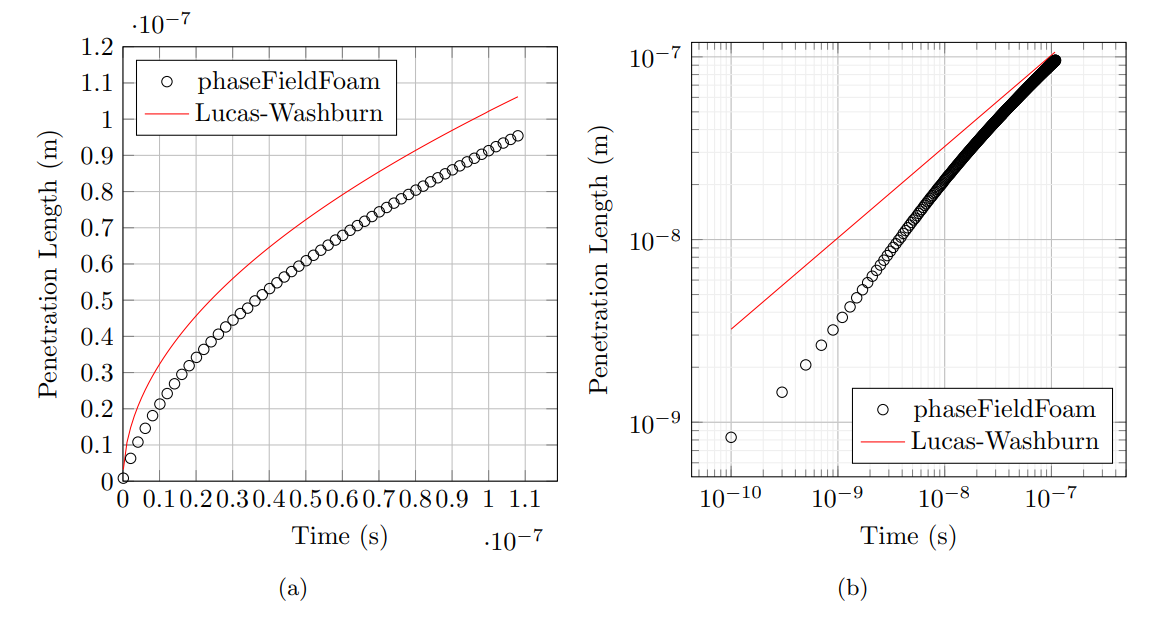
\includegraphics[width=.95\textwidth]{Pictures/LW-PFF_comp.png}
    \caption{Vergleich des von Lucas-Washburn vorhergesagten Wachstums mit den Ergenissen von \texttt{phaseFieldFoam}}
    \label{fig: LW-PFF_comp}
\end{figure}
In Abbildung \ref{fig: LW-PFF_comp} (a) wurde linear und in \ref{fig: LW-PFF_comp} (b) logarithmisch skalliert. In der logarithmischen Darstellung werden die Unterschiede deutlich sichtbar. Zu Beginn ist die Steigung der Simulationen größer als die der vorhersage, bis sie sich schließlich annähern. Das lässt darauf schließen, dass der Kapillare Aufstieg erst nach einiger Zeit dem bekannten Lucas Washburn Wachstum folgt, was auch der Aussage vieler in Abschnitt \ref{sec: capillaryRise} vorgestellter Arbeiten folgt. 

Um zu verstehen wieso das Verhalten sich unterscheidet, macht es Sinn sich die wirkenden Kräfte in der Wassersäule anzuschauen. Delanoy et al. \cite{delannoy2019DualRoleViscosity} führte diese unterschiede auf eine lokale Dissipation zurück. Daher macht es Sinn sich den Bereich nahe des Interfaces genauer anzuschauen. In Abbildung \ref{fig: viscForce-PFF} sind in (a) die viskosen Kräfte in der Wassersäule gezeigt. Es ist deutlich zu erkennen, dass nahe der Kontaktlinieam größten sind und sich entlang der wand \todo{ausarbeiten+ Bild nachbearbeiten. }

In Abbildung \ref*{fig: Velofield_Wedge} ist das Geschwidigkeitsfeld im Wasser dargestellt und sieht aus wie erwartet. In der Mitte der Kapillare ist die Geschwindigkeit des Wassers am höchsten (vgl. (a)). Zur Visualisierung des sich verändernden Geschwindigkeitsfeldes bei annäherung an das Interface wurden ebenfalls für drei Ebenen die Vektoren des Geschwindigkeitsfeldes hinzugefügt. Weit vom Interface entfernt, liegt das erwartete parabolische Profil vor. Bei näherung an das Interface ist deutlich zu erkennen wie die Strömung in der Mitte abgebremst wird und bei genauer betrachtung ist anhand der Vektoren auch zu erkennen, dass die Strömung an den Rand abgelenkt wird. Dazu wurde in (b) der Ausschnitt nahe des Interface vergrößert und statt der Magnitude der Geschwindigkeit nur die Komponente normal zur Strömungsrichtung ($z$-Richtung) visualisiert. Es ist deutlich zu erkennen, dass bis kurz vor der Strömung diese Komponente vernachlässigbar ist und nahe des Interface stark ansteigt und zwei Regionen zu bilden scheint. Eine direkt am Interface und nahe der Wand und ein weiteres etwas weiter innerhalb der Wassersäule. Anahnd der Legende ist deutlich erkennbar, dass die Größenordnung im Vergleich zur Geschwindigkeit in Strömungsrichtung sich um eine Dekade unterscheidet. Der Bereich in dem die Änderung der Geschwindigkeit stattfindet, wir im folgenden als $\mathrm{W}$ bezeichent.
\todo{Woher kommt das?}
\todo{Bild oder beschrieben der rezikulation} 

\begin{figure}[h]
    \centering
    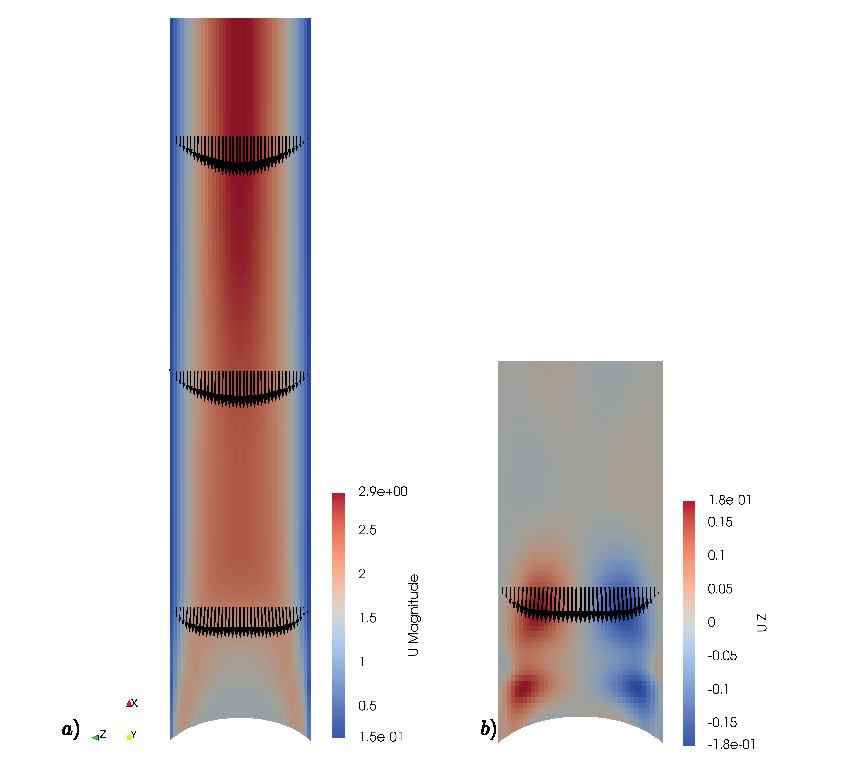
\includegraphics[width=.95\textwidth]{Pictures/Velo_Wedge.pdf}
    \caption{(a) Velocity field in the water column at $100ns$ and $\theta_{\mathrm{e}}=15^{\circ}$, (b) detailed view of recirculation near the interface.}
    \label{fig: Velofield_Wedge}
\end{figure}
In diesem Bereich ist nicht nur das Geschwindigkeitsfeld interessant. Schaut man sich die viskosen Kräfte in diesem Bereich (vgl. \ref*{fig: eDiss_wedge}) an, wird deutlich, dass sich zwei dissipative kanäle bilden. Die viskosen Kräfte nahe der Kontaktlinie und der viskosie Widerstand, hervorgerufen durch die Veränderungen des Kontaktwinkels aufgrund der Dynamik des Systems.

\begin{figure}[h]
    \centering
    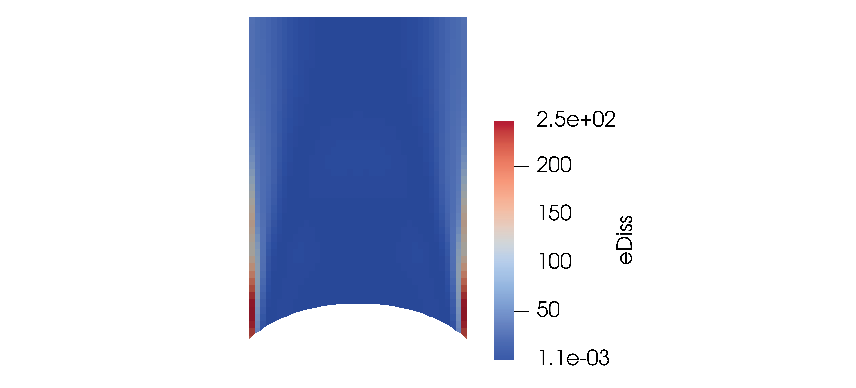
\includegraphics[width=.95\textwidth]{Pictures/eDiss_Wedge.pdf}
    \caption{Dissipative channels near the contact line.}
    \label{fig: eDiss_wedge}
\end{figure}

Zur Berechnung des Kontaktwinkels kann die in \ref*{chap: Validation} vorgestellte Methode zur Berechnung des Radius der spähre verwendet werden. Wie in Kapitel \ref*{chap: wettingTheory} beschrieben wird davon ausgegangen, dass sich der Meniskus zu einem Kreissegment entwickelt. Da in diesem Fall nur der Kontaktwinkel benötigt wird, kann auf eine in \cite{buttPhysicsChemistryInterfaces} vorgestellt Gleichung zurückgegriffen werden, womit sich der Kontaktwinkel mit 
\begin{equation}
    \theta = 90^{\circ}- 2\tan^{-1}\left(\frac{h}{R}\right) 
\end{equation}
berechnen lässt. Die variablen und wie sie erhalten werden ist bereits in Kapitel \ref*{chap: Validation} beschrieben. \todo{add cox angles to compare in one plot and just 15deg case}
\begin{figure}[h]
    \centering
    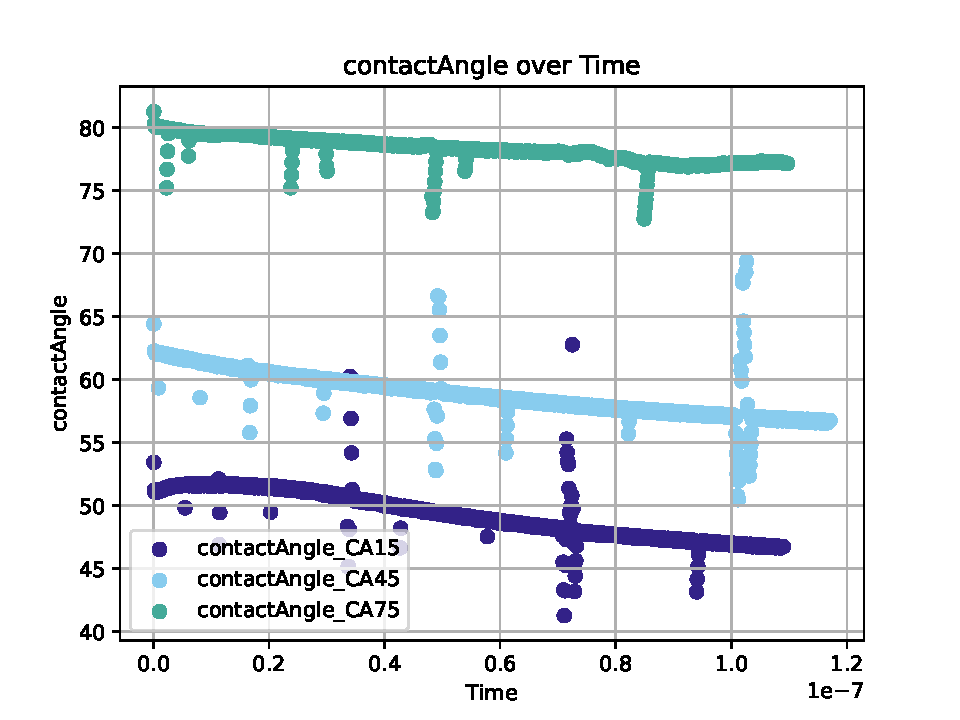
\includegraphics[width=.95\textwidth]{Pictures/contactAngle_overTime.pdf}
    \caption{computed contact angle over time }
    \label{fig: eDiss_wedge}
\end{figure}
Darin ist zu sehen, dass sich sehr schnell ein Winkel einstellt,... \todo{ausformulieren mit Daten vom feineren Netz.}

Die viskosen Kräfte ausserhalb von $\mathrm{W}$ werden aufgrund des Strömungsprofils als poiseuilles viskosen Widerstand angenommen. Um die in $\mathrm{W}$ herrschenden viskosen Kräfte zu ermitteln, wird von den insgesamt herrschenden viskosen kräften (Gleichung \ref*{eq: total_viscForce}) der Poiseuille Widerstand ($F_{\eta}$ aus Gleichung \ref*{eq: NewtonBalanceForcesOnly}) abgezogen. 
Weiter wird auch die aus Gleichung \ref*{eq: meniscusFormation} entstehenden Kräfte mit Hilfe der Simulation berechent. Plottet man diese Kräfte in einem Diagramm wird deutlich, wie zu Beginn der imbibition die Kräfte aus der Meniskusbildung die viskosen Kräfte überwiegen und erst nach einiger Zeit die viskosen Kräfte dominant werden. Dazu wurden in Abbildung \ref*{fig: forcesOverTime} auch die Ergebnisse aus der theoretischen Berechnung anhand der Simulationsdaten und der direkt aus der Simulation stammenden Daten gezeigt. Delanoy hat postuliert, dass ab einer imbibitionslänge von $\sim r\cdot ln(r/l_s)$ die viskosen Kräfte überwiegen. Auf diesen Fall übertragen würde das bedeuteten, dass für $t\approx 3\cdot 10^{-9}$ die viskosen Kräfte überwiegen. Da dies mit einer Automatischen auswertung der Ergebnisse nicht übereinstimmt, wurde exemplarisch für einen Fall händisch für mehrere Zeitschritte der Bereich $\mathrm{W}$ bestimmt und die Kräfte erneut überproft, wodurch sich dann nurnoch eine 


\begin{figure}[h]
    \centering
    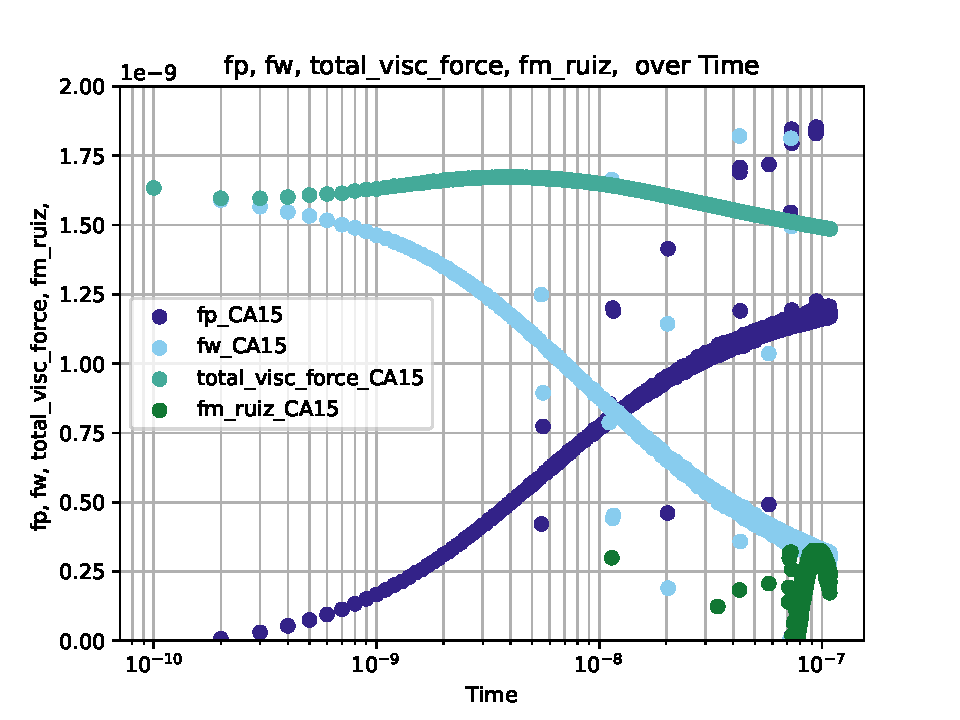
\includegraphics[width=.95\textwidth]{Pictures/log_fp_fw_total_visc_force_fm_ruiz_overTime.pdf}
    \caption{computed contact angle over time }
    \label{fig: forcesOverTime}
\end{figure}
%Diese erkenntnis bestätigt sich, wenn man die Steigung der SImulaiton an einigen Stichproben ermittelt. Dabei wird deutlich, dass die Steigung asymptotisch %auf den Wert der Lucas-Washburn Gleichung zustrebt. \todo{add table with slope values for some probes}




\section{Contact Angle Variation}
Wie zuvor erwähnt wurden die Simulationen für mehrere Kontaktwinkel durchgeführt, um mögliche Einflüsse bewerten zu können. Es ist zu erwarten, dass der Kontaktwinkel einen einfluss auf die Geschwindigkeit hat, mit der die Wassersäule aufsteigt. Dies zeigt sich auch in den Daten; auf eine darfstellung wird jedoch aufgrund der geringen aussagekraft verzichtet. Interessanter ist ein Vergleich der Kräfte, genauer eine Betrachtung der Anteile der Kräfte. Bildet man wie zuvor die Viskosen Widerstandskräfte und beziegt diese auf die ingesamt wirkenden viskosen Kräfte. Liegt dieses Verhältnis näher bei $1$, folgt der Kapillare aufstiegt dem Lucas-Washburn gesetzmäßigkeiten, für Werte nahe $0$, einem linearen Wachstum. Die darstellung über die Zeit zeigt, dass mit verändertem Gleichgewichtskontaktwinkel die Zeit beeinflusst wird, bis die viskosen Kräfte überwiegen. Es zeigt sich jedoch auch, dass der Kontatkwinkel bezogen auf die notwendige Strecke, die der Meniskus zurücklegt keinen Einfluss zu haben scheint. Dies spiegelt sich auch in der von Delanoy vorgeschalgenen formel zur Abschätzung des Punktes wieder an dem die viskosen Kräfte überwiegen.




\section{out of equilibrium boundary condition}
Bisher wurden alle auswertungen der Simulationen ohne die annahme einer Diffusion an der Wand und damit der annahme einer ideal Glatten Wand. In Abbildung \ref{fig: HDT_MKT_comp} (c) wurde eine molekulare wand illustriert. Trotz der angedeuteten unebendheiten würde diese wand vermutlich bereits einer ideal glatten wand gleichen. Allein aufgrund der tatsache, dass atome rund sind, kann keine ideal glatte ebene existieren. Eine simulation auf atomarer Ebene ist mit großem aufwand verbunden und um effekte der Wand dennoch abbilden zu können wurde in abschnitt \ref{sec: nonEquiBC} die Ungleichgewichtsrandbedingung eingeführt. Mit dem vorgestellten Faktor kann die Rauigkeit der Wand modelliert werden, desto größer der Wert, desto geringer die modellierte Dissipation an der Wand. 



\section{Conclusion}

EVERYTHING IS SHIT!!!!!!!!
I GIVE UP